\section{Felhasználói felület}
\subsection{Bejelentkezés}
Mielőtt bármilyen oldalt elérhetnénk, azonosítani kell magunkat, azaz be kell lépni az alkalmazásba. Az alábbi oldal az alapértelmezett főoldal:
\begin{figure}[h]
    \centering
    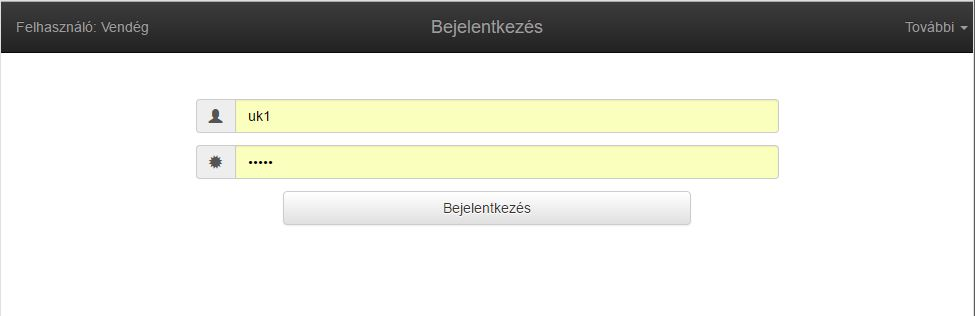
\includegraphics[width=16cm]{login.JPG}
    \caption{a bejelentezés}
\end{figure}
\\
Az oldal legfelső sávjában egy navigációs terület, amely a felhasználása során végig jelen lesz, viszont minden egyes oldalnak a hozzá megfelelő menüpontokkal. Ez a felsőléc három részre tagolódik. A tagolást a középen megjelenő oldal címe adja alapul. A címtől balra helyezkedik el és mindig megjelenik a Felhasználó: név címke, ahol a név a bejelentkezett felhasználói nevet takarja. Emelett itt még pár olyan menüpont jelenik meg, amely egy bizonyos felhasználói csoporthoz tartozik (lásd üzletkötő, illetve adminisztrátor, aki a felvett rendeléseket adminisztrálja, illetve továbbküldi kiszedésre és szállításra). A jobb oldalon egy lenyíló menü található, amelyben számos a felhasználó csoportoknál nagyjából megegyező menüpontok érhetőek el.

Itt több opció is megjelenik, viszont ha rá szeretnénk navigálni, akkor ugyanúgy a főoldalt fogja betölteni az alkalmazás, hiszen amíg az adott session nem azonosította magát, addig nem engedélyezett a további oldalak elérése. Ez szerver oldalon megírt kód, amelyhez felhasználtam a Scala Secured nevezetű interfészét, amelyet felüldefiniáltam. Ebben az interfészben négy darab metódus található: felhasználó lekérése, nem azonosított felhasználók átirányítása, azonosított felhasználók ellenőrzése, illetve egy metódus, amely ellenőrzi, hogy az adott felhasználónak van-e joga az adott oldalt elérni. Ez utóbbit részletezném kicsit, hisz minden oldalt szolgáltató response metódus ezt használja.
\begin{minted}{scala}
  def withUser(t :String)(f: User => Request[AnyContent] => Result) =
        withAuth { username => implicit request =>
    UserDAO.getUserByUserName(username).map { user =>
      if(user.accountType.equals(t)) {
        f(user)(request)
      } else {
        onUnauthorized(request)
      }
    }.getOrElse(onUnauthorized(request))
  }
\end{minted}
Itt a withUser nevű metódus látható, amely paraméterként egy felhasználói típust kér, ez az adott oldalhoz tartozó jogosultság csoport. Ez egy csomagoló függvény, amely ellenőrzi az előfeltételeket, majd az ellenőrzés kimenetének megfelelően vagy meghívja az f függvényt, amely a sikerességét jelzi az ellenőrzésnek, vagy az onUnauthorized függvényt, amely a felhasználót a bejelentkezési oldalra irányítja. A munkám során, így minden olyan response-ba, ahol azonosítanom kell, hogy a felhasználó jogosult-e azon oldal meglátogatására, ott elég csak a következőt alkalmaznom:
\begin{minted}{scala}
def függvénynév(paraméterek) = withUser{username => implicit request =>
    a megfelelő dolgok és a response.
}
\end{minted}
Ez nagy segítséget nyújt a kéretlen felhasználók ellen, és hogy minden felhasználó csak a saját funkcióit érhesse el.

\subsection{Főoldal}
A főoldal eléréséhez egy bejelentkezés szükséges, ennek részleteit az előző alfejezetben ismertettem. A bejelentkezés után az alábbi kép tárul elénk:
\begin{figure}[h]
    \centering
    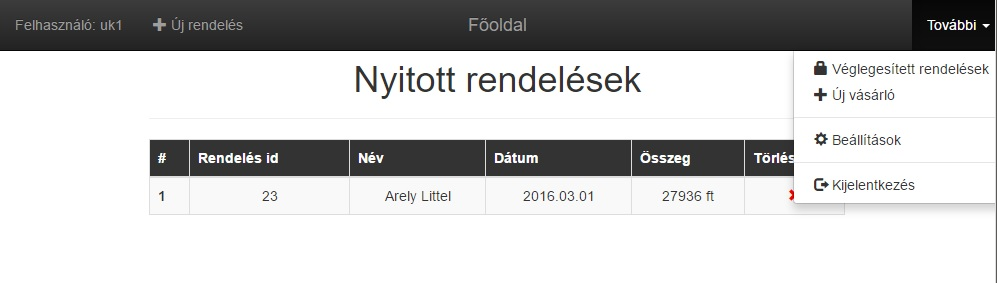
\includegraphics[width=16cm]{main.jpg}
    \caption{a főoldal}
\end{figure}
\\
A főoldal kettős jellegű hiszen ugyanaz a struktúra jelenik meg mind az adminisztrátoroknak illetve a felhasználóknak is, viszont a középen megjelenő táblázat és a menüpontok eltérnek. Míg az üzletkötőknek azon rendelések jelennek meg, amelyet felvettek, de még nem véglegesítettek az adminisztrátorok, addig az adminisztrátoroknak minden felhasználó által felvett rendelés megjelenik, amelyet ő törölhet illetve lezárhat, vagy megnézheti a termékeket. A táblázat minden sora egy-egy rendeléshez tartozik, és minden sor az adott rendelés részleteinek oldalára navigál. Az admin felületen a táblázat AJAX-os kéréssel frissül ki, amely azt jelenti, hogy miután betöltődött az oldal, egy újabb request érkezik a szervernek, amely konkrétan ezt a táblázatot küldi ki. Ez azért kell, hogy bizonyos időközönként frissíteni tudjuk a táblázatot (pl: percenként), és így az adminisztrátor mindig látja a legújabb rendeléseket amiket fel kell dolgozni.

A felhasználóknál a felső navigációs menüpontban található egy "Új rendelés" opció, amellyel új rendelést tud felvenni, illetve adminisztrátornál a véglegesített rendelésekre tud rákeresni. Továbbá a jobb oldalon található legördülő menü az adminisztrátoroknál az alábbi opciókat tartalmazza: Felhasználók (lásd 3.2.8), Vásárlók(lásd 3.2.9), Termékek, míg a területi képviselőknél, pedig Véglegesített rendelések, illetve Új vásárlók menüpontot. A Beállítások és Kijelentkezés opciók egyformán megtalálhatóak mindkét csoportnál.

A menüpontokhoz tartozó iconokat, a Bootstrap szolgáltatta. Ezek használat nagyon egyszerű ezt az Új rendelés menüponttal szemléltetem: 
\begin{minted}{html}
<span class="glyphicon glyphicon-plus"></span> Új rendelés
\end{minted}

\subsection{Új rendelés}
Ezen opció alatt a következő oldal jelenik meg:
\begin{figure}[h]
    \centering
    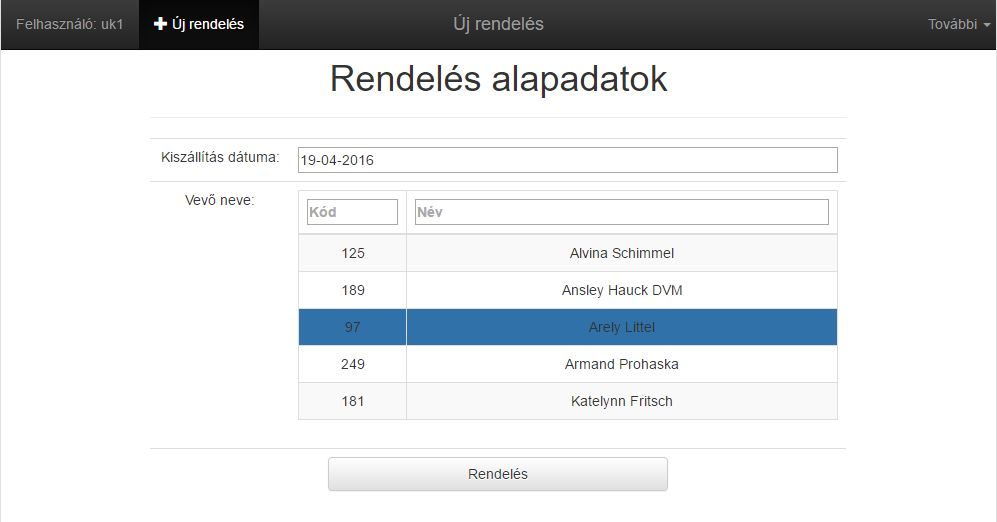
\includegraphics[width=16cm]{neworder.JPG}
    \caption{Alapadtok megadása: a kiválasztott vásárló kék szinnel jelölődik.}
\end{figure}
\\
A rendelési alapadatok rögzítésére szolgál a következő oldal. Megadható a vásárló, akinek szeretnénk rendelést felvenni. Itt mindig öt vagy kevesebb vásárló jelenik meg. A Kód, illetve Név mezőben írva, egy szűrés hajtódik végre. Mivel a kód az egyedi azonosítója a vevőnek, így ott egy pontos szűrés megy végbe, tehát az adott vásárló kilistázódásához be kell írni a teljes kódot. A név mivel nem feltétlen egyedi, keresés során a megadott karakterlánccal kezdődő vásárlókat listázza ki. Egy vásárló, akkor van kiválasztva, ha a sor bekékül(3.3 ábra). Az oldal betöltésekor egyetlen vásárló sincs kiválasztva. A táblázat itt is az AJAX-os request segítségével frissül, viszont itt minden másodpercben van egy lekérés, amelyet JavaScriptes időzítővel oldottam meg.

A kiszállítási dátum megadásához egy JavaScriptes dátum kiválasztót használtam, amely a következőképp jelenik meg: 
\begin{figure}[h]
    \centering
    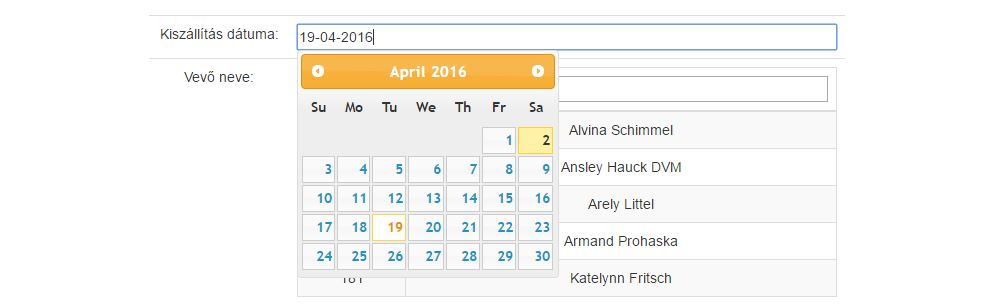
\includegraphics[width=16cm]{neworder2.JPG}
    \caption{időkiválasztás}
\end{figure}
\newpage
Majd ha mindkét adatot rendben megadtuk, akkor a Rendelés gomb segítségével tovább navigálhatunk a Termékek hozzáadása oldalra.
\subsection{Termékek hozzáadása}
A termékek hozzáadása oldal a következőképp jelenik meg:
\begin{figure}[h]
    \centering
    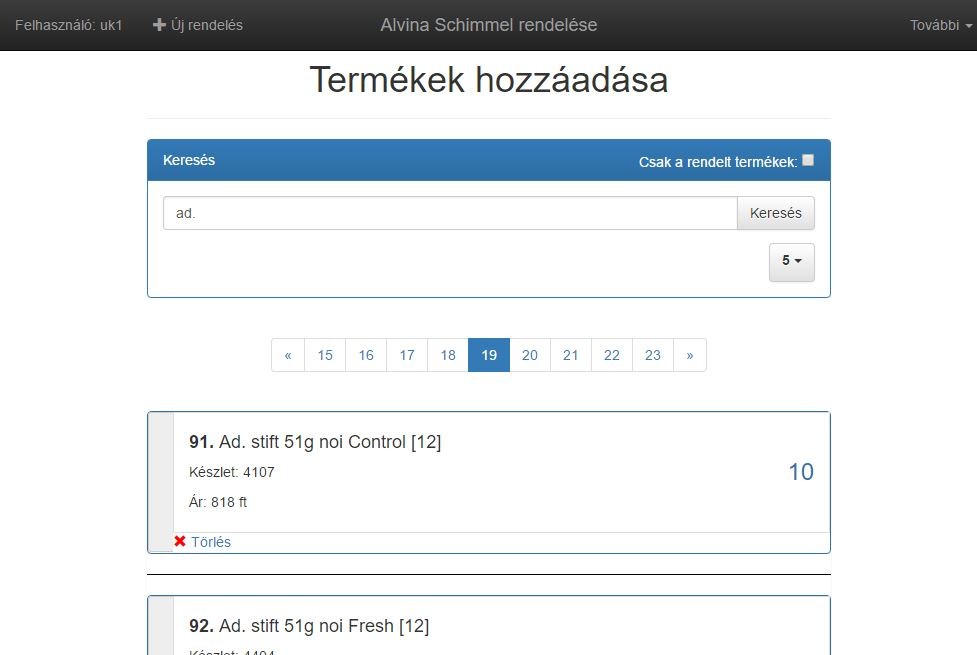
\includegraphics[width=16cm]{addorder.JPG}
    \caption{termékhozzáadás}
\end{figure}
\\
A felső sáv középpontjában a vásárló nevét láthatjuk, akihez a rendelés tartozik. A termékek keresése egy külön részt definiáltam, amelyben található egy input mező, amellyel termékekre kereshetünk név szerint. Továbbá itt található még egy "checkbox", ami segítségével eldöntheti a területi képviselő, hogy csak a már megrendelt termékeket listázza ki, illetve minden terméket. A termék keresést elősegítendő még egy oldalankénti termék számot megjelenítő legördülő menü. 
Az oldal érdekessége, hogy a termékeket megjelenítő rész, egy különálló részként van definiálva, amelyet majd több helyen fel fogok még használni. Ide tartozik a lapozás is, amely dinamikusan változik annak függvényében, hogy az adott keresésre hány darab elemet talált. A mezőkben megtalálható a termék neve, készlet szám és az ára, továbbá, a rendelt darab szám is. Ezen felül, a rendelt termékeknél megjelenik még egy törlés funkció is, amellyel kinullázhatja a megrendelt darabszámot. A darabszám hozzáadásához és a termék további részleteinek kilistázásához a Bootstrap modal nevezetű eszközét használtam, amely lényegében egy lebegő div (3.6-os ábra).
\begin{figure}[h]
    \centering
    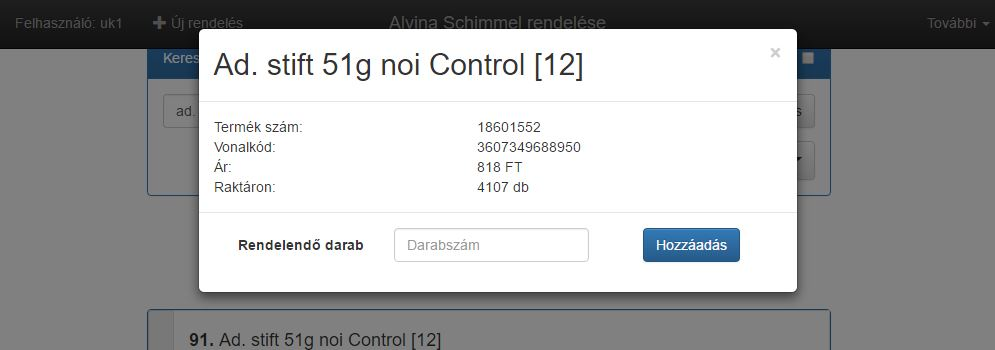
\includegraphics[width=16cm]{addorder2.JPG}
    \caption{Modal}
\end{figure}\\
Ez a div is hozzátartozik a termékeket megjelenítő részhez, egy egységet alkotva könnyedén felhasználható majd a nyitott rendelések menüpontban.
\subsection{Nyitott rendelések}
Miután felvettünk egy rendelést, sokszor úgy adódik, hogy azt később is módosítanunk kell, akár több terméket rendelnek, akár kevesebbet. Erre mindaddig van is lehetőségünk, amíg az adminisztrátor le nem zárja az adott rendelést. 
\begin{figure}[h]
    \centering
    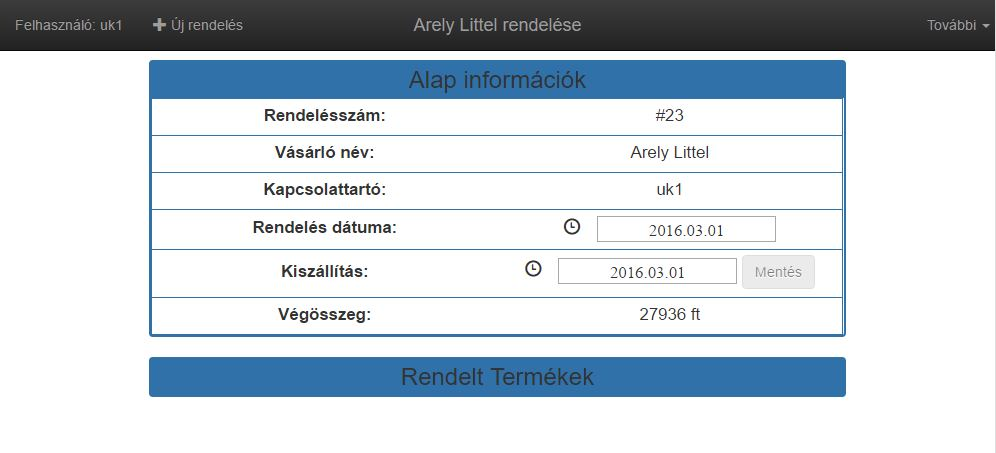
\includegraphics[width=16cm]{openorders.JPG}
    \caption{nyitott rendelések}
\end{figure}\newpage
A 3.7-es ábrán, látható, hogy az oldal két részre tagolódik. A két fő rész: az "Alap információk" és  a "Rendelt Termékek". Ez a két rész két "div"-ben található. Ezeknek van egy-egy fejléc mezőjük, amely kattintható, és ezen műveletre az aktuális rész láthatóvá vállik, a másik rész eltűnik. Mint már említettem, az alkalmazás mobil környezetben is elérhető, így fontos a hely takarékosság.

Az "Alap információk" részben, bizonyos információkat tudunk meg az adott rendelésről (pl: rendelésszám, vásárló név, kapcsolattartó, stb.). Ugyanakkor itt nem csak információkat kapunk, hanem módosíthatunk is. A kiszállítás dátumát tudjuk változtatni. Ezen művelet alapjául is egy JavaScriptes időkiválasztó gondoskodik, viszont itt csak azokat a napokat lehet bejelölni, amelyek az adott nap után vannak, hisz a kiszállítás nem tud a múltban megtörténni. Továbbá kezelve a felhasználók változatosságát, mindaddig amíg nem változtatunk a dátumon, addig nem tudunk a Mentés gombra kattintani. Ez segít elkerülni a felesleges request-eket. Ez egyszerűen egy JavaScriptes css állítással oldottam meg.

A "Rendelt Termékek" részben ugyanaz az oldal jelenik meg, mint a 3.2.4 fejezetben. Ahogy már ott említettem, ez egy különálló egységként működik (modul), így bárhova könnyedén beilleszthető. Itt pontosan ennek az előnyét használtam ki. Ahhoz, hogy ez egy Scala-s html-es vázból felépíthető legyen, ismét AJAX-os lekérést használtam. Ezen módszer segítségével egységessebb kinézetet és használatot biztosítok.

A nyitott rendelésekre, nem csak az üzletkötő kíváncsi, hanem az adminisztrátor is, hiszen innen tudja, hogy ki, mit rendelt, mit kell kiszállítani. Itt is próbáltam egységes maradni, így ugyanilyen kettős tagolás jellemző az adminisztrátori "Nyitott rendelések" oldalra is. Viszont az egyes részek bővültek, illetve módosultak.

Az "Alap információk"-nál, már a kiszállítás dátumán nem tudunk változtatni, hiszen ez egy ajánlott kiszállítási dátum, amelyet nem feltétlen kell betartani. Továbbá megjelenik a "Kiszedett összeg" mező is, amely azt tárolja, hogy a szállításra kiszedett termékek pontosan mennyibe fognak kerülni. \newpage
\begin{figure}[h]
    \centering
    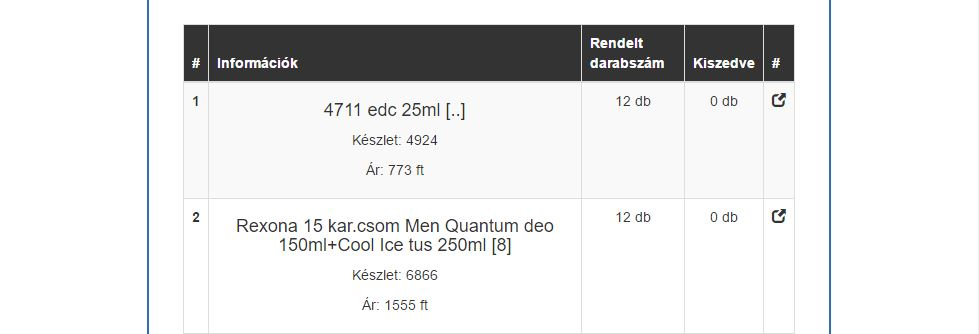
\includegraphics[width=16cm]{openorders2.JPG}
    \caption{Rendelt termékek adminisztrátori szemszögből.}
\end{figure}
A "Rendelt Termékek" résznél, némiképp változott a termékek listázása. Itt egy táblázat jelenik meg, amelynek utolsó oszlopában, megjelenik egy "Összes kiszedése" szimbólum, amely arra szolgál, hogy ha az adott termékből a rendelni kívánt mennyiség került kiszedésre és szállításra. Itt ha az oszlop soraira navigálunk, akkor előugrik, egy már ismert modal (3.6-os ábra), csak itt a kiszedésnek megfelelő input mezőkkel. Ott be tudjuk írni, hogy hány darab az, amely kiszedésre került. Mindkét művelet során, a raktáron lévő darabszám csökken, illetve, ha kiszedünk egy terméket, de mégse szerettük volna, akkor visszaírjuk, és így nem csökken hanem nő. Ezek segítségével, egy közel valós raktáron lévő darabszámot tudunk kiállítani. \\
Ha minden terméket kiszedettnek talál az adminisztrátor, akkor a főoldalon tudja nyugtázni és véglegesíteni a rendeléseket.

\subsection{Véglegesített rendelések}
Miután az adminisztrátor véglegesít egy nyitott rendelést, az a véglegesített rendelések között fog megjelenni. Ez a menüpont megegyezik, mind az adminisztrátorok, mind az üzletkötők szempontjából. 
\begin{figure}[h]
    \centering
    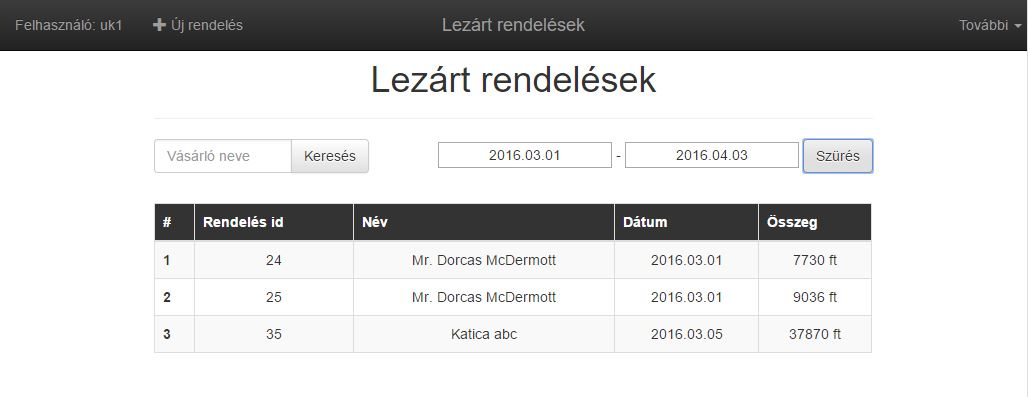
\includegraphics[width=16cm]{closedorder.JPG}
    \caption{Rendelt termékek adminisztrátori szemszögből.}
\end{figure}\\
Mivel véglegesített rendelés mennyisége nagy lehet, így alkalmazni kellett egy időbeli szűrést a megjelenítésénél. Itt kiválaszthatjuk, hogy mely időszakot jelenítse meg. Alapértelmezetten ez a szűrés 10 napra visszamenőlegesen van beállítva.\\
Továbbá lehetőségünk van név alapján keresni. Ez a két feltétel külön szűrést alkalmaz, így ha beállítunk egy adott időintervallumot, akkor visszakapjuk a kezdő időponttól a vég időpontig a lezárt rendeléseket, míg névre az adott karakterlánccal kezdődő összes véglegesített rendelést.

Minden egyes táblázat sorral elnavígálhatunk a sorhoz tartozó lezárt rendelés részletező oldalára. Itt szinte ugyanaz a kép tárul elénk, mint a 3.7-es ábrán található adminisztrátori szemszögből, annyi különbséggel, hogy itt nem tudunk módosítani semmit, hiszen ezt a rendelést már kiszállították. A "Rendelt Termékek" részben ugyanazon egység található, mint az adminisztrátorok nyitott rendelések menüpontjában, itt is azon kivétellel, hogy módosítani nem tudunk semmit. Így a táblázat utolsó sora se jelenik meg, továbbá a modal-ban sem jelenik meg az input mező.
\subsection{Felhasználók módosítása}
Ez a menüpont csak az adminisztrátoroknak jelenik meg. Ők vesznek fel új üzletkötőket vagy akár adminisztrátorokat a rendszerbe. Ez a lista számosságát tekintve, ahogy már említettem 5-50 körülire becsülhető, a cégek nagyságát tekintve. Alapértelmezetten az admin felhasználó van létrehozva a programhoz, és neki van jogosultsága több felhasználót felvenni a rendszerhez. Továbbá, ha admin jogú felhasználót hoz létre, ő is megkapja ugyanazon jogokat.
\begin{figure}[h]
    \centering
    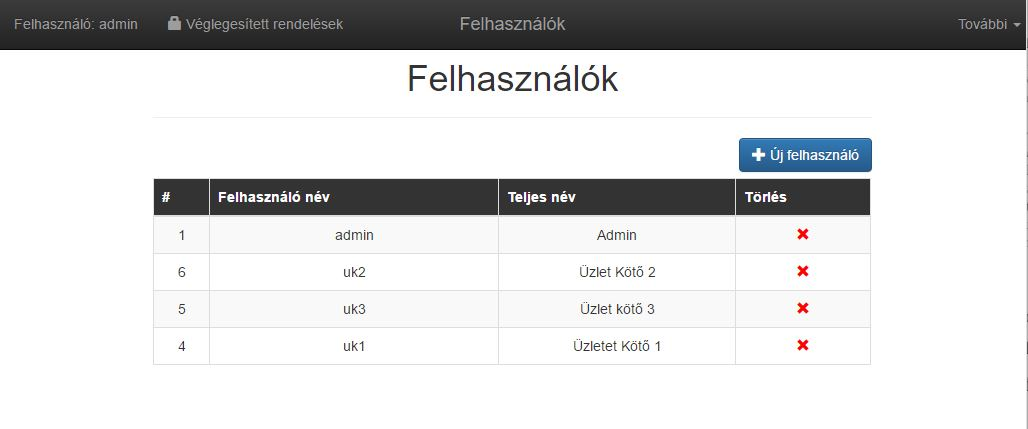
\includegraphics[width=16cm]{usersmodify.JPG}
    \caption{felhasználók módosítása}
\end{figure}\\
A felhasználók listája egy táblázatban jelenik meg, melynek minden sora az adott felhasználó egyedi oldalára navigál, ahol módosíthatjuk az adataikat. Jelenleg a felhasználó nevet, teljes nevét és a jelszót tudja módosítani az admin. A jelszó módosítása css-ben letiltható, viszont úgy találtam, hogy vész esetére az adminok segítenek, az elfelejtett jelszó átállításában.

Az oldalon található még egy Új felhasználó gomb is, amely segítségével, ugyanarra a form-ra navigál minket az oldal, mint ha egy felhasználóra klikkel, viszont itt minden mező üresen lesz hagyva. Így a felhasználók kezelése is egységes marad.

Felhasználókat nem csak hozzá tudunk adni a rendszerhez, hanem törölni is, hiszen bármikor megszűnhet egy bizonyos pozíció. Erre ad lehetőséget a táblázat utolsó sora, ahol-is egy piros x látható.

A felhasználók egyediségét biztosítja a felhasználói név egyedisége, továbbá található mellettük egy egyedi azonosító is. Ha a módosítások, illetve új felhasználó felvétele során egyediségi megszorításnak nem teszünk eleget, akkor egy hiba üzenet fog megjelenni a Mentés gomb alatt és a módosítások nem mentődnek el.
\subsection{Vásárlók módosítása}
A felhasználók módosítása menüpont alatt található táblázatos megjelenítés itt is előtűnik. Ellenben, mivel a vásárlók száma több száz, akár több ezer is lehet, itt mindenféleképpen kell alkalmazunk, valamilyen szűrést, illetve lapozást. A szűrés név szerint valósul meg, igaz a vásárlóknál, ez nem egyedi azonosító, de a táblázatban kilistázódik a Kód száma is, amellyel együtt már egyedivé vállik egy vásárló. 
\begin{figure}[h]
    \centering
    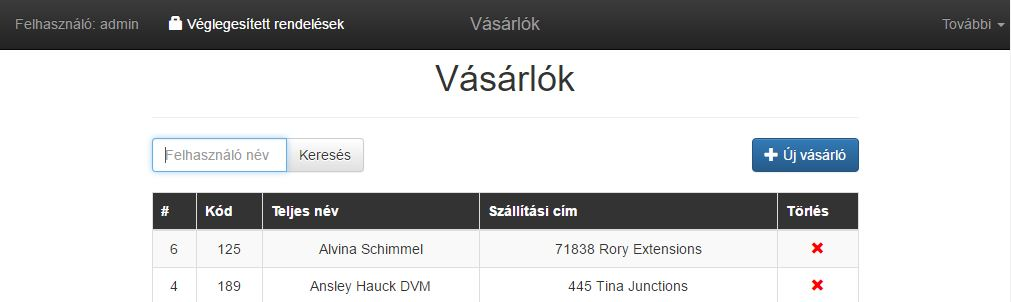
\includegraphics[width=16cm]{customers2.JPG}
    \caption{vásárlók módosítása}
\end{figure}\\
A táblázat sorai ismét egy-egy vásárló adataira navigálnak minket, ahol természetesen módosíthatjuk is azokat, kivéve az egyedi generált kód számát. Itt is megjelenik egy Új vásárló nevezetű gomb, amely ugyanazon az elven működik, amelyet már leírtam a 3.2.7-es alfejezetben, csak itt vásárlókra nézve.\\
Ezen oldalhoz tartozik még egy funkcionalitás is. Ez pedig az új vásárlói kérelmek elfogadása. Az adminisztrátor segítségével tartjuk karban, hogy a rendszerben, csak valódi vásárlók kerüljenek be.
\begin{figure}[h]
    \centering
    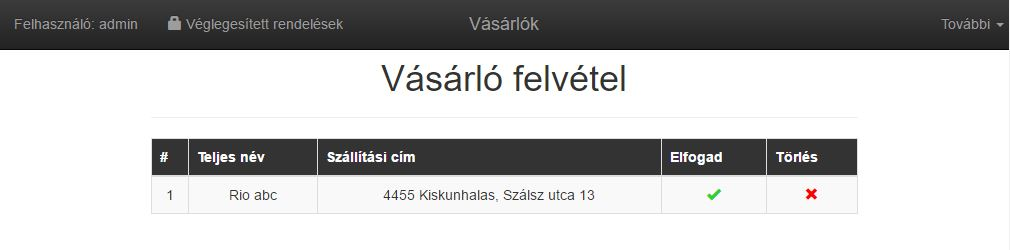
\includegraphics[width=16cm]{customers.JPG}
    \caption{vásárlók módosítása}
\end{figure}\\
Az oldal tetején, a vásárlók előtt jelenik meg a vásárló felvételi táblázat, ahol kilistázódik az összes új vásárló, akiket az üzletkötők szeretnének hozzáadni. A táblázat utolsó két sorában található a pipa azaz az elfogad, illetve az x azaz elutasítás. Ezen táblázat sora nem kattintható, viszont elfogadás után bekerül a vásárlók táblázatba, és ott bármikor módosítható lesz. Itt is fent áll a lehetőség az automatikus megjelenítésre, hiszen egy különálló "div"-ben jelenik meg a vásárló felvétele, így az bármikor megjeleníthető JavaScript-ből, a teljes oldal kifrissítése nélkül.

\subsection{Új vásárló felvételének kérelme}
Az alkalmazás törekszik, hogy minden lehetséges funkcionalitást megadjon a felhasználóinak, az egységes kommunikációra. Ez a menüpont is ezért készült el, hisz így az alkalmazáson belül küldhetünk egy új vásárlói kérelmet, amelyet az adminisztrátornak el kell fogadnia. Így megkönnyíti mind az adminisztrátorok és az üzletkötők munkáját is. Ez a menüpont csak a területi képviselők számára érhető el.
\begin{figure}[h]
    \centering
    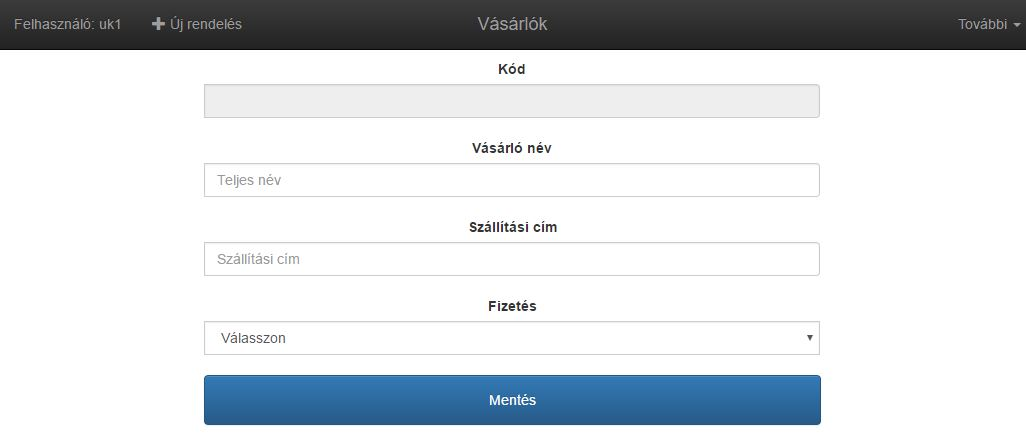
\includegraphics[width=16cm]{newcustomerrequest.JPG}
    \caption{új vásárló felvételének kérelme}
\end{figure}\\
A form hasonlít a vásárlók és a felhasználók form-jára. Itt nem találunk egyediségi megszorítást, hiszen ahogy már említettem, a vásárló neve nem egyedi, az a kóddal együtt válik azonosítóvá.
\newpage
\subsection{Termékek módosítása}
\begin{figure}[h]
    \centering
    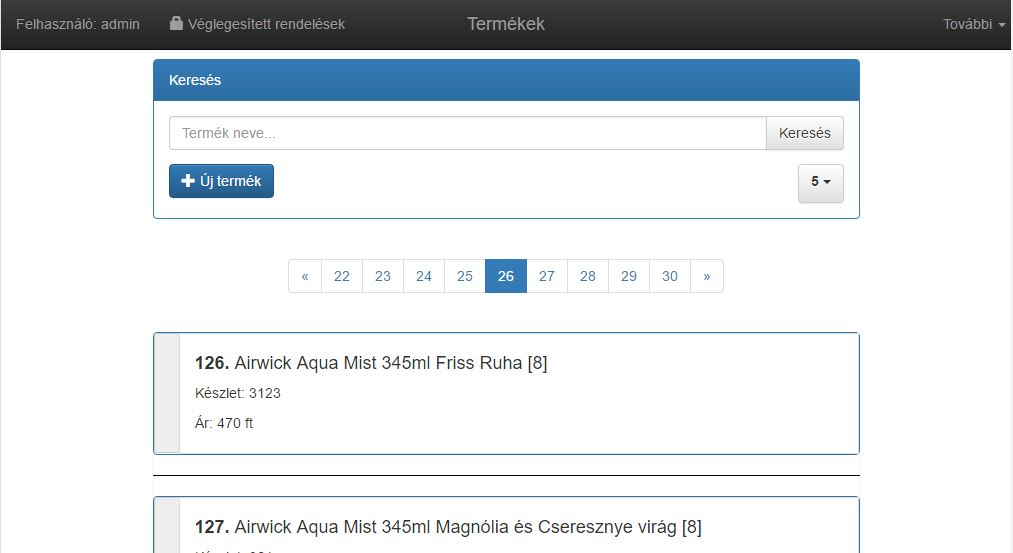
\includegraphics[width=16cm]{products.JPG}
    \caption{új vásárló felvételének kérelme}
\end{figure}\\
A termékek hozzáadása, és módosítása menüpont alatt, az egységesség jelében ugyanazon oldal struktúrával találkozunk, mint mikor termékeket adunk egy rendeléshez. Viszont itt megjelenik egy Új termék gomb, amely segítségével új terméket adhatunk a mostani adatbázisunkhoz. Itt is a vásárlók és felhasználók módosításánál használt módszert alkalmazom, azaz ugyanazon form jelenik meg, ha már meglévő termékre kattintunk, illetve újat veszünk fel, annyi különbséggel, hogy a termék adatok nem jelennek meg. 

Termékek törlésére a rendszer nem biztosít lehetőséget, hiszen lehet, hogy a véglegesített rendelések között megtalálhatóak a törölni kívánt termékek, és ha a termék törlődne, nem lehetne valós képet visszaállítani az adott rendelésről.
\newpage
